%==============================================================================
\chapter{Tips and tricks}
\label{sec:tips}\index{tips}
%==============================================================================

\LaTeX{} file: \url{./guide/guide_tips.tex}\\[1ex]
\noindent
Over time I have collected quite a lengthy list of things you should
\enquote{Do} and \enquote{Not Do} (at least in my head) that I think
it is useful to write down early in the document, so that you may
actually read them!  In this chapter I will first tell you how to get
and use the style file and then give some tips.

%------------------------------------------------------------------------------
\section{How to use the \Package{ubonn-thesis} style}
\label{sec:tips:howto}
%------------------------------------------------------------------------------

The idea with this document is that you also look at the \LaTeX{} that
is used to create it, in order to find out how things are done.
I will therefore usually not give the \LaTeX{} commands in the printed
document, but assume that you will have a look at the \LaTeX{} source.
To help you with this, each chapter contains a link to the relevant
file at the top. This link should work if you have compiled the guide
yourself and are in the \texttt{ubonn-thesis} directory.
The files that make up this document are available in a subversion
repository and as a \texttt{tar} file. To get the latest subversion
entries give the command:

\begin{verbatim}
svn co https://svn.physik.uni-bonn.de/basic/ubonn-thesis/trunk
\end{verbatim}
\noindent
If you want to checkout a particular release you can give the command:
\begin{verbatim}
svn co https://svn.physik.uni-bonn.de/basic/ubonn-thesis/tags/ubonn-thesis-N.M
\end{verbatim}
% \noindent
% If you have checked out a version of the guide before 20 August 2012
% and want to update things, you need to change the location:
% \begin{verbatim}
% cd ~/ubonn-thesis/trunk
% svn switch --relocate svn://svn.physik.uni-bonn.de/ubonn-thesis \
%  https://svn.physik.uni-bonn.de/basic/ubonn-thesis
% \end{verbatim}
\noindent
The tar file (and the release tree (as of release 1.5)) also includes
the guide as a PDF file: \texttt{thesis\_guide.pdf}.  It can be
obtained from:\\
\url{http://www-biblio.physik.uni-bonn.de/info/index.shtml#info:titelvorl}
and\\
\url{http://pi.physik.uni-bonn.de/pi_only/thesis.php}.

\par\noindent
Once you have the files, you can then give the command:
\begin{verbatim}
make new [THESIS=dirname]
\end{verbatim}
to create a new directory with a couple of files to help you get
started. By default the directory name will be \texttt{mythesis}.
If you choose a different name, you have to adjust the \Macro{include}
commands inside \texttt{./dirname.tex}.
To compile your thesis try:\index{compiling}
\begin{verbatim}
make thesis [THESIS=dirname]
\end{verbatim}

My original idea was that the style file should work for all recent
\TeX\ installations.  However, some of the packages I recommend have
been changing quite a lot over the past few years. By default things
should work with \TeXLive 2011 and later.\index{TeXLive@\TeXLive!2011}
If you have an older version, you should set the value of
\Macro{texlive} in the thesis main file to
2009\index{TeXLive@\TeXLive!2009} rather than 2011 and then use the
command \enquote{\texttt{make thesis09}} rather than
\enquote{\texttt{make thesis}}. Note that you should not mix these two
commands. If you switch from one to the other do a
\enquote{\texttt{make clean cleanbbl cleanblx}} in between.

\noindent
In the main thesis file, \texttt{mythesis.tex}, you need to specify
which cover page should be used:\index{cover page}
\begin{description}
\item[\texttt{PhD\_Submit\_Title.tex} and \texttt{PhD\_Final\_Title.tex}:]
  the title pages for a PhD thesis;\index{PhD}\index{thesis!PhD}
\item[\texttt{Master\_Submit\_Title.tex} and \texttt{Master\_Final\_Title.tex}:]
  the title pages for an MSc thesis;\index{MSc}\index{thesis!Master}
\item[\texttt{Diplom\_Submit\_Title.tex} and \texttt{Diplom\_Final\_Title.tex}:]
  the title pages for a Diplom thesis;\index{Diplom}\index{thesis!Diplom}
\item[\texttt{Bachelor\_Title.tex}:]
  the title pages for a BSc thesis.\index{BSc}\index{thesis!Bachelor}
\end{description}
For the printed version for the department library you also need to
include the appropriate cover page (with an abstract):\index{cover}
\begin{description}
\item[\texttt{PhD\_Cover.tex}:]
  The cover page for a PhD thesis;
\item[\texttt{Diplom\_Cover.tex}:]
  The cover page for a Diplom thesis;
\item[\texttt{Master\_Cover.tex}:]
  The cover page for an MSc thesis.
\end{description}
This extra cover should not be included for the version of the PhD
thesis that is submitted to the university library (ULB). See
Section~\ref{sec:tips:submit} for some more details.

If you are not a member of the
\foreignquote{ngerman}{Physikalisches Institut} you should
also change \Macro{InstituteName}, \Macro{inInstitute} and
\Macro{InstituteAddress}. The style file \texttt{ubonn-thesis.sty}
already contains the appropriate definitions for PI, HISKP, IAP and
AIFA.

All packages that are needed should be part of your \TeX\
installation. If not you may have to install them or ask your system
administrator to do so.

If you just want to make the cover pages, use the file
\texttt{cover\_only.tex}.  Be sure to adapt the font selected in
\texttt{ubonn-thesis.sty} to the font you actually used in your
thesis. Be aware that not all font sizes are available in all font
collections. If you used the default \LaTeX{} font in your thesis,
then choose \Package{lmodern}\index{font!lmodern} in the style file.

The main file for this guide is \texttt{thesis\_guide.tex} and it
includes the \LaTeX{} files in the directory \texttt{./guide} and the
Feynman graphs in the directory \texttt{./feynmf}. Again this guide
should compile without changes for \TeXLive 2011. For earlier versions
set \Macro{texlive} in \texttt{thesis\_guide.tex} to
2009.\footnote{You should set \Macro{texlive} to 2011 also if you have
  \TeXLive 2012,\index{TeXLive@\TeXLive!2012} which is the default
  version for Ubuntu 12.10.\index{ubuntu!12.10}}


%------------------------------------------------------------------------------
\section{Do}
\label{sec:tips:do}
%------------------------------------------------------------------------------

\begin{itemize}
\item Have 1--2 other people read your thesis well before you are
  supposed to submit it. Do not ask too many; everyone has their own
  opinions on how things should be written, how much detail should be
  included etc.\ and these opinions will not necessarily agree with
  each other!
\item Write \enquote{nice} \LaTeX. It makes it much easier to find mistakes
  in your document. If you like to use the keyboard rather than the
  mouse when moving round in a document, turn on \enquote{auto-fill-mode
  (emacs)}\index{emacs} or its equivalent in any other editor, so
  that line breaks are inserted.
\item Make sure every table and figure is referenced in the text. I
  get very irritated when I suddenly find a figure that is not
  described in the text.
\item Use a units package to format numbers and their units. Recent
  versions of \LaTeX\ include the \PackageG{siunitx} package, which
  is a superior replacement of \Package{SIunits}. I used to
  use \Package{SIunits}, or rather \Package{hepunits} which is
  built on top of \Package{SIunits}, and defines common particle
  physics units such as \si{\GeV}. Use of these packages will be
  discussed in Section~\ref{sec:tips:units}. An alternative is the
  \Package{units} package.
\item Define any complicated symbols once you use them more than
  once:
\begin{verbatim}
\newcommand{\etajet}{\ensuremath{\eta_{\text{jet}}}\xspace}
\end{verbatim}
  If you decide at a later date that jet should be a superscript
  rather than a subscript you only have to change this in one place!
\item If you use normal words in superscripts or subscripts (or
  anything else in math mode) enclose them in \Macro{text}. You can
  also use \Macro{mathrm} or \Macro{textrm}. However, if you then use
  the same symbols in slides with a sans-serif font, the text may well
  continue to be in a
  serif font.\\
  {\sffamily Compare: A common jet energy cut at the LHC is now
    $p_{T}^{\text{jet}} > \SI{20}{\GeV}$, while at HERA we typically
    \ifthenelse {\texlive = 2009} {%
      used $p_{T}^{\mathrm{jet}} > \SI[obeyfamily=false]{6}{\GeV}$.
    }{%
      used $p_{T}^{\mathrm{jet}} > \SI[detect-family=false]{6}{\GeV}$.
    }}
  The \si{\GeV} in the first expression is in sans-serif. This is
  because the
  \Macro{sisetup}\texttt{\{detect-family=true\}}\footnote{\Option{obeyall}
    in \TeXLive 2009.} option is set in \texttt{ubonn-thesis.sty}
  (see Section~\ref{sec:tips:siunitx}).  I used the option
  \Option{detect-family=false}\footnote{\Option{obeyfamily=false} in \TeXLive
    2009} for the \Macro{SI} command in the 2nd expression.
  In the first expression I use \Macro{text} for \enquote{jet}, while
  I use \Macro{mathrm} in the second expression.
\item Use \Macro{xspace} and
  \Macro{ensuremath} in all commands where you would
  like to use a symbol both in text mode and in math mode. Without
  \Macro{xspace} you have to make sure that you end every symbol with
  \texttt{\textbackslash} or \texttt{\{\}}, otherwise the space is used
  to signify the end of the symbol, e.g. in \LaTeX we have to pay
  attention otherwise the symbol and the next word run together.
\item Decide how you want to write abbreviations for particles and
  stick to it -- you should probably define the particle names in your
  style file and always use them (also for quarks). At some point the
  CERN Computer Newsletter claimed that all particle should be written
  upright, e.g. $\text{Z}$ boson, $\text{b}$ quark. However, nowadays
  it seems to be much more common to use math mode. This is also how
  the particles are written in the PDG. I would therefore
  recommend one of the following definitions:
\begin{verbatim}
\newcommand*{\Zo}{\ensuremath{Z}\xspace}
\newcommand*{\Zo}{\ensuremath{\text{Z}}\xspace}
\newcommand*{\bbarQ}{\ensuremath{\bar{b}}\xspace}
\newcommand*{\bbarQ}{\ensuremath{\bar{\text{b}}}\xspace}
\end{verbatim}\index{particles}
  which produce \ensuremath{Z}, \ensuremath{\text{Z}},
  \ensuremath{\bar{b}}, \ensuremath{\bar{\text{b}}}. Note that you are
  not allowed to include numbers in the names of commands, so
  \Macro{Z0} or \Macro{U1S} are not valid commands. For
  $\overline{B}^{\pm}_{c}$ and other particles whose names are capital
  letters, it can be debated whether it better to use
  \Macro{overline} than
  \Macro{bar}. Compare $\overline{B}^{\pm}_{c}$ and
  $\bar{B}^{\pm}_{c}$. If you use upright letters the choice is maybe
  easier: $\overline{\text{B}}^{\pm}_{\text{c}}$ and
  $\bar{\text{B}}^{\pm}_{\text{c}}$ or
  $\overline{\text{K}}^{0}_{\text{S}}$ and
  $\bar{\text{K}}^{0}_{\text{L}}$.

  Note that Kopka~\cite{kopka04}
  recommends using \Macro{newcommand*} rather than \Macro{newcommand}
  for short commands.
\item Decide how you want to write coordinate axes\index{coordinates}
  and stick to it. Far too often I see text like: \enquote{The proton
    beam defines the Z direction, while the interaction point is
    denoted as $(x_{0}, y_{0}, z_{0})$. The polar angle is measured
    with respect to the z axis and $\cot\theta = p_{Z}/\pT$}. Which is
  the best way of writing the coordinates? As $x$, $y$ and $z$ are
  often used for kinematic variables, there are arguments in favour of
  $(X, Y, Z)$.
\item Use \Macro{enquote} from the \PackageG{csquotes} package to
  quote text rather than using explicit quotation marks. This has the
  advantage that consistent quotation marks are used everywhere (also
  if they are nested) and that they are also correct for the language
  (and dialect\footnote{%
    By default, British English\index{British English}\index{UK English}
    uses `British quoted text' for outer quotation marks,
    while American (US) English\index{American English}\index{US English}
    uses \foreignquote{USenglish}{American quoted text}. In this guide
    (and in \texttt{ubonn-thesis.sty})
    \foreignquote{USenglish}{American (US) quotes} are used even if you
    write in British (UK) English.})  you are writing your thesis in. You
  can also see in the Chapter~\ref{sec:intro} how this works, even
  when switching languages inside a paragraph.
\item Use sizes that depend on the font size, \texttt{em}\index{em}
  (width of \enquote{M}) and \texttt{ex}\index{ex} (height of \enquote{x}), for
  spacing that should change with the text size. Use absolute sizes
  \texttt{cm, mm, pt} etc.\ where they are appropriate, e.g.\ title
  pages, boxes, etc. \Macro{quad} and
  \Macro{qquad} are also useful sizes in tables and
  equations.
\item Add a \textbackslash{} (or \{\}) after abbreviations that end with a full
  stop such as e.g.\ if followed directly by text. If you do not, an
  end of sentence space is added rather than a normal interword
  space. Note that \textbackslash{} is not needed (but does no harm)
  after abbreviations that only consist of capital letters:\\
  compare \enquote{e.g. my name is Ian C. Brock}
  and \enquote{e.g.\ my name is Ian C.\ Brock},
  where \textbackslash{} was included in the second version. In this
  example the difference is small. However, if \LaTeX{} increases the
  spacing between words to fill a line the effect is more obvious.
\item Ask someone (me) if you cannot easily find out how to solve
  formatting problems. I recently saw a thesis in German, where the
  author wanted to use commas instead of full stops in numbers and
  wrote numbers as \verb+$2,\!47$+ to produce $2,\!47$ instead of
  $2,47$. There are usually much better solutions, e.g.\
  \verb+\num{2.47}+ with the \Package{siunitx} package produces
  \num{2.47} in English and \foreignlanguage{ngerman}{\num{2.47}} in
  German. In the end such solutions will save you time!
\item Use punctuation in equations and \enquote{\dif}, i.e.\ \Macro{dif} for
  derivatives,\index{derivative} e.g.
  \begin{equation*}
    \int y\, \dif x\,.
  \end{equation*}
  This is also one of the the very few places, where it makes sense
  to put some spacing in by hand -- normally you should leave this to \TeX.
\item Pay attention to the alignment of numbers in
  tables. \Package{siunitx} provides the \Option{S} column specifier to
  help with this. Packages such as \Package{dcolumn} also provide assistance.
\end{itemize}

Not really a strict \enquote{Do}: I highly recommend that you use an
integrated environment for editing and compiling your thesis. If you
are on a Mac or under Windows you probably use TEXshop or
\TeXLive. Under Linux you can use Kile\index{kile} or the way I work
is to use \texttt{emacs}\index{emacs} and AUCTeX. Note that the
RefTeX\index{RefTeX} mode in \texttt{emacs} also provides powerful
tools for finding cross-references and the names of citations
easily. \TeXstudio is based on \TeXmaker and is available for Linux,
Windows and MacOSX. One advantage of such environments is that it is usually
possible to switch between a position output and the relevant place in
the source code and vice versa. This makes it much quicker to fix
things when you spot an error in your output PDF file. You can usually
also step through the errors when you try to compile your file and fix
them directly. In addition, they know which environments and
mathematical symbols exist, which can speed things up if you have not
been working with \LaTeX\ for the past 20 years!

More details on installing \TeX\ for different systems can be found
in Appendix~\ref{sec:app:tex}.


%------------------------------------------------------------------------------
\section{Do Not}
\label{sec:tips:dont}
%------------------------------------------------------------------------------

\begin{itemize}
\item Don't write symbols differently in math mode and in text. One of
  my pet hates is:
  \enquote{The most famous equation in the world is:
  \begin{equation}
    \label{eq:emc2}
    E = m c^{2}
  \end{equation}
  where E is the energy of the particle and m is its mass}, i.e.\ $E$
  and $m$ are in math mode in the equation, but in text mode in the
  text where they are explained.
\item Another example of how not to write things is something like
  \enquote{The scale factor, SF, used to correct the MC is determined in
  an independent dataset using $SF = N_{data} / N_{MC}$}. Note the
  wrong font and spacing of $SF$, $data$ and $MC$. All should be
  enclosed in \Macro{text}: $\text{SF} = N_{\text{data}} / N_{\text{MC}}$.
\item Do not include the directory or the extension of the file in
  \Macro{includegraphics}
  commands. Use
  \Macro{graphicspath}
  instead to set up a list of directories that hold the
  figures.\index{figures!directories} Let \LaTeX{} or PDF\LaTeX{} pick
  the extension for the figure, so that you can (in principle) easily
  switch between the two.
\item Do not try to end paragraphs with
  \textbackslash\textbackslash. These should be used sparingly when
  for some reason you really have to start a new line. Just leave an
  empty line for a new paragraph.
\item Do not draw conclusions or interpret figures in the caption. The
  caption should just describe what is in the figure. Interpretation
  belongs in the main body of the text.
\item Do not start trying to format figure and table captions inside
  each caption -- use the options available in \KOMAScript{} to set
  such things at the beginning of the document.
\item Do not worry about overfull boxes, positions of figures
  and tables, etc.\ until you reach the final version of your thesis.
\end{itemize}


%------------------------------------------------------------------------------
\section{Units}
\label{sec:tips:units}\index{units}
%------------------------------------------------------------------------------

As just mentioned above, but I'll say it again just to make the point,
one of my pet hates is inconsistent and poor typesetting and spacing
of units. At least three standard packages exist to solve this
problem: \Package{siunitx}, \Package{SIunits} and \Package{units}. My
favourite is \Package{siunitx} as it offers many extra features in
addition to the correct typesetting of numbers and their units.

Instead of \Package{SIunits}, I used to use \Package{hepunits}, which
is based on \Package{SIunits} but includes units commonly used in
particle physics such as \si{\GeV} and \si{\pico\barn}. Unfortunately
the syntax of the \Package{hepunits} and \Package{units} packages is
different even though they use the same macro name. In
\Package{hepunits} you write \verb+\unit{10}{\GeV}+, while in
\Package{units} you write \verb+\unit[10]{\GeV}+. The
\Package{siunitx} package is quite new and older versions were
supposed to have compatibility modes for both \Package{SIunits} and
\Package{units}, but I had problems getting them working. It uses the
macros \Macro{SI} and \Macro{num} rather than \Macro{unit}.


%------------------------------------------------------------------------------
\subsection{siunitx package}
\label{sec:tips:siunitx}\index{siunitx}

This package is a more modern and complete package than either
\Package{SIunits} or \Package{units}. As the package is rather new it
is also still developing. There are quite a few changes from version 1
(\TeXLive 2009)\index{TeXLive@\TeXLive!2009} to version 2 (\TeXLive
2011)\index{TeXLive@\TeXLive!2011} which means that several of the
examples I include here have somewhat different syntaxes depending on
which version of \TeXLive is being used to compile this guide. If you
use \TeXLive 2011, but want to use units which were available in
\TeXLive 2009 or the older syntax you can include the option
\Option{version-1-compatibility}. Note that \TeXLive 2009 was the
default version for Ubuntu releases up to and including
12.04,\index{ubuntu!12.04}. I will give the \Package{siunitx} version
2 options in the text and the version 1 options as footnotes.

One very attractive feature is that it allows you to format
computer-generated numbers such as \verb+1.4E4+ automatically,
e.g. \verb+\num{1.4E4}+ produces \num{1.4E4}. Depending on the
language or using the option
\Option{exponent-product}\footnote{\Option{expproduct} in \TeXLive
  2009.} you can also get
\ifthenelse {\texlive = 2009} {%
  \num[expproduct=cdot]{-3.4E-6}.  }{%
  \num[exponent-product=\cdot]{-3.4E-6}.
}
It is even possible to set
the number of decimal places, cf.\ \SI{2.99467E8}{\metre\per\second}
and
\ifthenelse {\texlive = 2009} {%
  \SI[dp=1]{2.99467E8}{\metre\per\second}, }{%
  \SI[round-mode=places,round-precision=1]{2.99467E8}{\metre\per\second},
}
which only differ by the use of the \Option{round-mode} and
\Option{round-precision}\footnote{\Option{dp} in \TeXLive 2009}
options, and even rounds correctly!

Another extremely nice feature of the package is that you can typeset
numbers in a single way and then a full stop or a comma will be used
as the decimal point, depending on which language you set for your
document. This means that computer generated decimal numbers can be
output with commas in a German thesis just by changing the language of
your thesis -- this for me is \LaTeX{} at its best! For example,
writing \verb+\num{1.2345E-3}+ produces \num{1.2345E-3} in the default
language of the document and
\foreignlanguage{ngerman}{\num{1.2345E-3}} if I say that this piece of
text is in German (\Option{ngerman} to be exact).

In keeping with \LaTeX{} philosophy, you can specify a number and its
error using \verb+\num{2.88(32)}+ to produce \num{2.88(32)} with the
\Option{separate-uncertainty}\footnote{\Option{seperr}
  in \TeXLive 2009.} option (which I specify) or $2.88(32)$ with the
default option. You also give as an option how units with negative
powers of units should be shown, e.g.\ per second. This can be changed
for a single command.

Some examples are given below:
\begin{itemize}\setlength{\itemsep}{0pt}\setlength{\parskip}{0pt}
\item $c$ is \SI{3E8}{\metre\per\second} -- default \Macro{per};
\item $c$ is
\ifthenelse {\texlive = 2009} {%
  \SI[per=fraction,fraction=nice]{3E8}{\metre\per\second}
}{%
  \SI[per-mode=fraction,fraction-function=\sfrac]{3E8}{\metre\per\second}
}
  -- using \Option{per-mode=fraction,fraction-function=\Macro{sfrac}}\footnote{%
    \Option{per=fraction,fraction=nice} in \TeXLive 2009}
\item written in \Env{displaymath} or preferably \Env{equation*}:
\ifthenelse {\texlive = 2009} {%
  \begin{equation*}
    c = \SI[per=slash]{2.99E8}{\metre\per\second}
  \end{equation*}
}{%
  \begin{equation*}
    c = \SI[per-mode=symbol]{2.99E8}{\metre\per\second}
  \end{equation*}
}
with \Option{per-mode=symbol}\footnote{%
  \Option{per=slash} in \TeXLive 2009};
\item $\hbar$ is \SI{1.054E-34}{\joule.\second}.
\end{itemize}
You use \enquote{.} or \enquote{,} to make a space between the units,
as illustrated in the last bullet.
Angles are also very straightforward -- just use \Macro{ang} as in
\ang{90}.

If you also want to use \Package{siunitx} in slides, where one usually
uses a sans serif font, you may at first be disappointed that
\Package{siunitx} uses a serif font for the units! DO not despair!
You can use the command
\Macro{sisetup}\texttt{\{detect-family=true\}}\footnote{\Option{obeyall}
  in \TeXLive 2009.} to ensure that the package uses the current font
(in all its aspects) rather than its default.

Have a look at the manual, \texttt{texdoc siunitx}, for many more
examples. \Package{siunitx} also contains useful and powerful tools
for typesetting tables and as mentioned above can be used to round
numbers. These aspects are discussed in Chapter~\ref{sec:table}.

Note that the \Macro{clight} symbol that is used in the macro
\Macro{MeVovercsq} to produce \si{\MeVovercsq} is defined as $c_{0}$ in
\Package{siunitx} version 2. As this is not the way it is usually
written in high energy physics I redefined it using:
\begin{verbatim}
  \DeclareSIUnit\clight{\ensuremath{c}}
\end{verbatim}

Two things that are currently not built in are separate statistical and
systematic errors and asymmetric errors. From the author I got some
suggestions on how to define such things. They are included in
\texttt{guide\_defs.sty} at present and can be added to
\texttt{thesis\_defs.sty}. Two versions of a few of the commands are
defined depending on the value of \Macro{texlive}, as some of the
options changed when moving from version 1 to version 2 of
\Package{siunitx}. Several new macros have been defined there:
\Macro{numerrt}, \Macro{numpmerr} and \Macro{numpmerrt} to write
errors with a description, which are asymmetric and both,
respectively. The corresponding macros for values and errors are
\Macro{SIerrt}, \Macro{SIpmerr} and \Macro{SIpmerrt}. For the macros
whose names end with \enquote{\texttt{t}}, you also have to provide
the descriptive text. If you have two errors then use \Macro{SIerrtt}
or \Macro{SIpmerrtt}, which have two or three more arguments,
respectively. For the standard case of statistical and systematic
errors, you can use the macros \Macro{SIerrs} and
\Macro{SIpmerrs}. Examples of their use are:
\begin{itemize}
\item $\sigma = \SIerrs{3.42}{0.46}{0.32}{\pico\barn}$
\item $\sigma = \SIpmerr{3.42}{0.46}{0.32}{\pico\barn}$
\item $\sigma = \SIpmerrt{3.42}{0.46}{0.32}{\stat}{\pico\barn}$
\item $\sigma = \SIpmerrs{3.42}{0.46}{0.32}{0.06}{0.04}{\pico\barn}$
\item $\sigma = \SIpmerrtt{3.42}{0.46}{0.32}{\stat}{0.06}{0.04}{\sys}{\pico\barn}$
\end{itemize}
The last two examples use \Macro{SIpmerrs} and \Macro{SIpmerrtt} just
to show that they can both give the same output. If you need even more
complicated combinations of errors, or more errors, have a look at the
definitions, e.g.
\begin{equation*}
  \sigma_{t\bar{t}} = (\num{164.6}%
  \valuesep\numerrt{8.7}{\stat}%
  \valuesep\numpmerrt{6.4}{5.3}{\sys}%
  \valuesep\numerrt{8.2}{lumi.})%
  \valuesep\si{\pico\barn}
\end{equation*}


%------------------------------------------------------------------------------
\subsection{SIunits/hepunits packages}
\label{sec:tips:siunits}\index{SIunits}\index{hepunits}

Before I found \Package{siunitx} these used to be my preferred units
packages.
% While \Package{siunitx} is supposed to have a compatibility
% mode for \Package{hepunits} I had problems getting this working.
This section therefore gives examples on how to use \Package{hepunits}
and what you should be careful about. As \Package{siunitx} has got
stricter about what it allows for a syntax, I have had to cheat in the
\LaTeX\ code several times to show the effect.

Even though \Macro{xspace} is used for some units in \Package{hepunits}
it does not appear to have the usual effect.
Hence, if you use units in normal text it is probably wise to
terminate them with \enquote{\textbackslash } or \enquote{\{\}}. Compare
\begin{itemize}
\item The \si{\GeV}is a
  heavily used unit in particle physics and cross-sections measured in
  \si{\pico\barn}or \si{\nano\barn}are quite common.
  Masses can be given in either \si{\MeVovercsq}or \si{\MeV}.
\item The \si{\GeV} is a
  heavily used unit in particle physics and cross-sections measured in
  \si{\pico\barn} or \si{\nano\barn} are quite common.
  Masses can be given in either \si{\MeVovercsq} or \si{\MeV}.
\end{itemize}
In the first bullet the units were not terminated, while in the second
they were.

Note that \Package{SIunits} typesets the value in text mode and the
unit in math mode. You only have to worry about this if you want to
use math mode symbols e.g. $10^{8}$ in the value. Three different ways
of writing the velocity of light are:
\begin{itemize}\setlength{\itemsep}{0pt}\setlength{\parskip}{0pt}
\item $c$ is \verb+\unit{$3 \cdot 10^{8}$}{\metre\per\second}+
\item $c$ is
  \verb+\unit{3$\cdot$\power{10}{8}}{\metre\reciprocal\second}+
\item $c$ is \verb+\unit{3 $\cdot$ \power{10}{8}}{\metre\usk\reciprocal\second}+
\item Written in \Env{displaymath} or preferably \Env{equation*}:
\begin{verbatim}
  \begin{equation*}
    c = \unit{$3 \times \power{10}{8}$}{\metre\usk\reciprocal\second}
  \end{equation*}
\end{verbatim}
\end{itemize}
Note the difference in spacing in the examples. The first
example gives the best result. Two different ways of handling the value
are used in the second and third examples, either without or with space between
the number and \verb+$\cdot$+. In the fourth example, where you use
\Macro{unit} in math mode, you still need to enclose the value in
\$...\$ if it includes characters from math mode.  Conversely if for
some reason you want normal text in your units, you should put it
inside \Macro{text}, e.g. the velocity of light is
$\SI{3E8}{\text{metres per second}}$. If you forgot the
\Macro{text} command using\\
\verb+\unit{$3 \cdot \power{10}{8}$}{metres per second}+ you would
get:
$3 \cdot 10^{8}\,metres per second$ or if you tried to write the units
yourself you would get $3 \times 10^8\,m s^{-1}$.

If you have negative powers then you can play around with
the \Macro{power} command and the usual superscript:
\begin{itemize}
\item $\hbar$ is \verb+\unit{$1.054 \times 10^{-34}$}{\joule\usk\second}+
\item $\hbar$ is \verb+\unit{1.054 $\times$ \power{10}{-34}}{\joule\usk\second}+
\item $\hbar$ is \verb+\unit{1.054 $\times$ \power{10}{$-34$}}{\joule\usk\second}+
\end{itemize}
Note the use of \Macro{usk} to get a bit of space between the
units. In the second example the minus sign appears as a dash,
\enquote{-}, rather than \enquote{$-$}, which is too small. Hence, if you
use \Macro{power} you should put the power in math mode.

Just to complicate things further, if you use the Palatino font for
example, then the standard \TeX{} font is used in math mode. You thus
have to decide from the very beginning whether numbers should
\textbf{ALL} be in text or in math mode. This is clearly one of the
disadvantages of using a font for which the math mode is different
from the text mode. ATLAS uses either the \Package{txfonts} or the
\Package{mathptmx} packages, which do not have this problem. This is
why I use \Package{txfonts} in this guide. If the numbers
$1234.56$ and 1234.56 look the same then you do not have to
worry! There are ways to get around the problem with Palatino. You can
try either the \Package{pxfonts} or the \Package{mathpazo} packages --
for my taste the sans serif font used in \Package{pxfonts} looks a bit better.


%------------------------------------------------------------------------------
\section{Hints}
\label{sec:tips:hints}
%------------------------------------------------------------------------------

\Package{xspace} is great, but how do you write $B^{0}\bar{B}^{0}$ when
you have defined the symbols \Macro{Bo} and \Macro{Bobar} with
\Macro{xspace} at the end. Here you need \verb+{}+ between the two
commands, e.g. \verb+\Bo{}\Bobar+ produces \Bo{}\Bobar while
\verb+\Bo\Bobar+ produces \Bo\Bobar.

How should you write \enquote{between $10^{4}$ and $10^{5}$}?\index{range}
If you use math mode it looks like $10^{4} - 10^{5}$, which is not
really what you want. Although it is rather clumsy, the best way to do
it is \verb+$10^{4}$--$10^{5}$+ which produces
\enquote{$10^{4}$--$10^{5}$}.

With \Package{siunitx} and \Macro{num} there
is a built-in option. You simply write\\
\verb+\numrange{3e4}{7e4}+
to produce \enquote{\numrange{3e4}{7e4}} or\\
\ifthenelse {\texlive = 2009} {%
  \texttt{\textbackslash SIrange[tophrase=-\,-]{5}{7}{\textbackslash GeV}}
  to produce \enquote{\SIrange[tophrase=--]{5}{7}{\GeV}}.
  If you only want the unit to appear once write\\
  \texttt{\textbackslash SIrange[range-units = single, tophrase=-\,-]\{5\}\{7\}\{\textbackslash GeV\}}
  to produce
  \SIrange[trapambigrange=false, tophrase=--]{5}{7}{\GeV}.
}{%
  \texttt{\textbackslash SIrange[range-phrase=-\,-]\{5\}\{7\}\{\textbackslash GeV\}}
  to produce \enquote{\SIrange[range-phrase=--]{5}{7}{\GeV}}.
  If you only want the unit to appear once write\\
  \texttt{\textbackslash SIrange[range-units = single, range-phrase=-\,-]\{5\}\{7\}\{\textbackslash GeV\}}
  to produce
  \SIrange[range-units = single, range-phrase=--]{5}{7}{\GeV}.
}
In a single range, such settings are rather long-winded!
However, they can be applied to the whole
document using the \Macro{sisetup} macro.

With \Package{SIunits} and \Macro{unit} you can write
\verb+\unit{\power{10}{4}--\power{10}{5}}{}+, which would look almost
correct, but leaves some space for the unit! If you want to write
between 5 and \SI{7}{\GeV}, then \Macro{unit} works well:
\verb+\unit{5--7}{\GeV}+.

A similar problem is how do you write \enquote{about 10\%}?  Again the
simple solution $\sim 10\%$ or $\sim$ 10\% have too much space. In the
file \texttt{thesis\_defs.sty} two macros \Macro{mysim} and
\Macro{mysymeq} are defined that add some negative space so that you
can simply put everything in math mode: $\mysim 10\%$ or $\mysimeq
0.2$. An alternative is to use \Macro{SI} or \Macro{unit}, as there
should actually be some space between the number and the \% sign,
e.g.\ \verb+$\sim$\SI{10}{\%}+, which produces $\sim$\SI{10}{\%}, is
completely correct and does not need the use of \Macro{mysim}.

What is the difference between \Macro{textrm} and
\Macro{mathrm}? I used to worry about this and found a
few examples (which I then forgot) where the font size was better
using one or the other. Then I learnt about \Macro{text},
converted all my predefined symbols to use \Macro{text} rather than
\Macro{mathrm} or \Macro{textrm}, and don't have to worry any
more. However, I can given an example: the transverse energy of the
highest energy jet is denoted $p_{T}^{\mathrm{1^{\text{st}} jet}}$ if
one uses \Macro{mathrm}, while it is denoted by
$p_{T}^{\textrm{1$^{\text{st}}$ jet}}$ if you use \Macro{textrm},
where I used \Macro{text} to produce $1^{\text{st}}$.  As you can see
from this example, the key difference is that \Macro{mathrm} switches
to an upright font, but keeps you in math mode -- hence ignoring any
spaces. \Macro{textrm} switches to text mode (with a serif font) and
therefore pays attention to spaces.

A perennial problem is bold math\index{math!bold} when it is needed in
section headings etc. This is further complicated by the fact that the
table of contents is usually not typeset using a bold font (except for
chapter titles, or whatever the highest level(s) of sectioning are.
The only reliable way to get this right in both cases is to give the
heading twice, once with \Macro{boldmath} for the real title and once
without as the optional title for the table of contents.  An
illustration of how this works is given in Appendix~\ref{sec:emc2}.


%------------------------------------------------------------------------------
\section{Submitting your thesis}
\label{sec:tips:submit}\index{submit}
%------------------------------------------------------------------------------

Questions often come up when your thesis is finished and now you have
to print it and submit it. Both the
\foreignquote{ngerman}{Promotionsbüro} and the
\foreignquote{ngerman}{Prüfungsamt} have instructions on what you have
to do, but it is sometimes not clear what this means in terms of the
cover pages offered by this thesis framework.

For the printed version of your thesis, you probably want
\Package{hyperref} links and the table of contents to be black. In
order to do this, you should uncomment the \Macro{hypersetup} command
that is in the thesis main file, just after the
\Macro{usepackage}\texttt{\{mythesis/thesis\_defs\}}.


%------------------------------------------------------------------------------
\subsection{PhD thesis}
\label{sec:tips:submit:phd}\index{submit!PhD thesis}\index{PhD}

\subsection{Submission}

\begin{enumerate}
\item Use the file \texttt{PhD\_Submit\_Title.tex} for the title
  pages. 
  This is selected by passing the options \Option{PhD, Submit}.
  to the \Macro{documentclass} or the \Package{ubonn-thesis} package.
  Leave the \foreignquote{ngerman}{Tag der Promotion} and
  \foreignquote{ngerman}{Erscheinungsjahr} blank.
\item You are required to also submit a CV\index{CV} and a summary of your
  thesis. A skeleton CV is provided as the file
  \texttt{thesis\_cv.tex} which you then include at the end of your
  thesis. The summary should also be printed separately.
\item You have to print and bind five copies of your thesis for the
  \foreignlanguage{ngerman}{Promotionsbüro}. Nowadays these are
  usually in colour.
  One of these copies will go to the department library.
\item The first and second referees for your thesis often like to also
  have an extra copy of the thesis so that they can make comments when they read
  your thesis --- ask them if they want one. You can usually save the
  institute some money and print these copies in black \& white.
  Some referees even prefer to get the extra copy as a PDF file.
\end{enumerate}


\subsection{Printing the final version}

\begin{enumerate}
\item Use the file \texttt{PhD\_Final\_Title.tex} for the title page.
  This is selected by passing the options \Option{PhD, Final}.
  to the \Macro{documentclass} or the \Package{ubonn-thesis} package.
\item Do not include your CV\@.
\item There are probably some small corrections you or the referees
  found during the time between submission and your examination. These
  should be corrected before you submit your thesis to the university
  library (ULB).\index{ULB}\index{university library}\index{library!university}
\item Almost everyone submits their thesis electronically to the ULB\@.
  You also have to print two copies for them.\footnote{%
  This used to be five, but was reduced in 2015.}
  The ULB is quite strict on the quality of the binding etc. The university
  print shop is not able to fulfil the requirements, so you have to print
  these versions externally. When you do this do not forget to
  uncomment the \Macro{hypersetup} command as mentioned above, if you
  want to print them in colour.
\item The department library\index{department library}\index{library!department}
  (in the Physikalisches Institut) needs seven printed copies with the file
  \texttt{PhD\_Cover.tex} as the cover and
  \texttt{PhD\_Final\_Title.tex} for the title pages.
  These are selected by passing the options \Option{PhD, PILibrary}
  to the \Macro{documentclass} or the \Package{ubonn-thesis} package.
  You have to get
  the \enquote{BONN-IR-YYYY-nnn} number from the librarian. You
  should also include an abstract (in English) on the cover page. You
  can also use this abstract when you submit your thesis
  electronically to the ULB\@.
\item The department library version of the thesis is the one that you usually print if
  you need extra copies for your experiment or research group.
\end{enumerate}

Note that when you want to get your degree certificate, you will get
some forms from the \foreignlanguage{ngerman}{Promotionsbüro} that have
to fill out.
These forms have to be signed by your supervisor.
One of the forms asks you if you have published significant parts of your
thesis elsewhere.
This means your actual thesis and not a paper that uses the results from your thesis.
If you submit your thesis electronically to the ULB, then you should not fill out this form.
It only applies if you actually publish your thesis elsewhere
(which is allowed by the \foreignlanguage{ngerman}{Promotionsordnung}).


Appendix~\ref{app:printer} suggests some printer shops that can make copies
of your thesis in good enough quality to be accepted by the university
library.


%------------------------------------------------------------------------------
\subsection{Master/Diplom/Bachelor thesis}
\label{sec:tips:submit:other}\index{submit!MSc thesis}\index{submit!Diplom thesis}\index{submit!BSc thesis}

\subsubsection{Submission}

\begin{enumerate}
\item Use the file \texttt{Master\_Submit\_Title.tex},\index{MSc}
  \texttt{Diplom\_Submit\_Title.tex}\index{Diplom} or
  \texttt{Bachelor\_Title.tex}\index{BSc} for the title pages.
\item You have to print and bind three copies of your thesis
  to be submitted to the
  \foreignlanguage{ngerman}{Prüfungsamt}. Nowadays these are usually in
  colour.
\item The first and second referees for your thesis often like to also
  have an extra copy of the thesis so that they can make comments when they read
  your thesis -- ask them if they want one. You can usually save the
  institute some money and print these copies in black \& white.
\end{enumerate}

Note that a CV does not to be included in a Master/Diplom/Bachelor
thesis. This is only needed when you submit a PhD thesis.


\subsubsection{MSc/Diplom theses for the department library}

\begin{enumerate}
\item Use the file \texttt{Master\_Cover.tex} for the cover and
  \texttt{Master\_Final\_Title.tex}\footnote{Replace Master with Diplom
    as appropriate.} for the title pages.
\item There are probably some small corrections you or the referees
  found during the time between submission and the completion of the
  referees' reports and grades. These should be corrected before you
  submit your thesis to the department library.
\item The department
  library\index{department library}\index{library!department} (in the Physikalisches
  Institut) needs 2 printed copies with the file\\
  \texttt{Master\_Cover.tex} as the cover. You have to get
  the \enquote{BONN--IB--YYYY--nnn} number from the librarian. You
  should also include an abstract (in English) on the cover page.
\item This version of the thesis is the one that you usually print if
  you need extra copies for your experiment or research group.
\end{enumerate}


\subsubsection{BSc theses}

\begin{enumerate}
\item There are probably some small corrections you or the referees
  found during the time between submission and the completion of the
  referees' reports and grades. These should be corrected before you
  print some extra copies of your thesis if your group wants them.
\end{enumerate}


%------------------------------------------------------------------------------
\section{Line numbering}
\label{sec:tips:lineno}\index{lineno}\index{line numbers}
%------------------------------------------------------------------------------

You probably do not need line numbers when writing your
thesis (who knows?). However, as this is a very useful package that
occasionally has some problems, I thought I would include some
information here.

\Package{lineno} is the package to use to get line numbers in your text,
but sometimes a block of lines is not numbered - see Fig.~\ref{fig:lineno}a.

\begin{figure}[htbp]
  \centering
  \begin{tabular}{cc}
  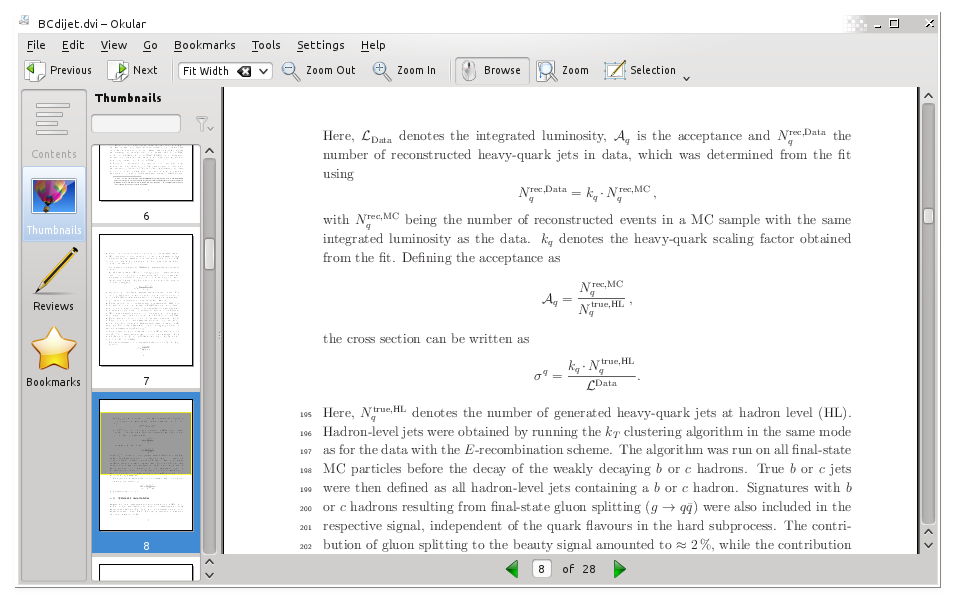
\includegraphics[width=7cm]{BCDijet} &
  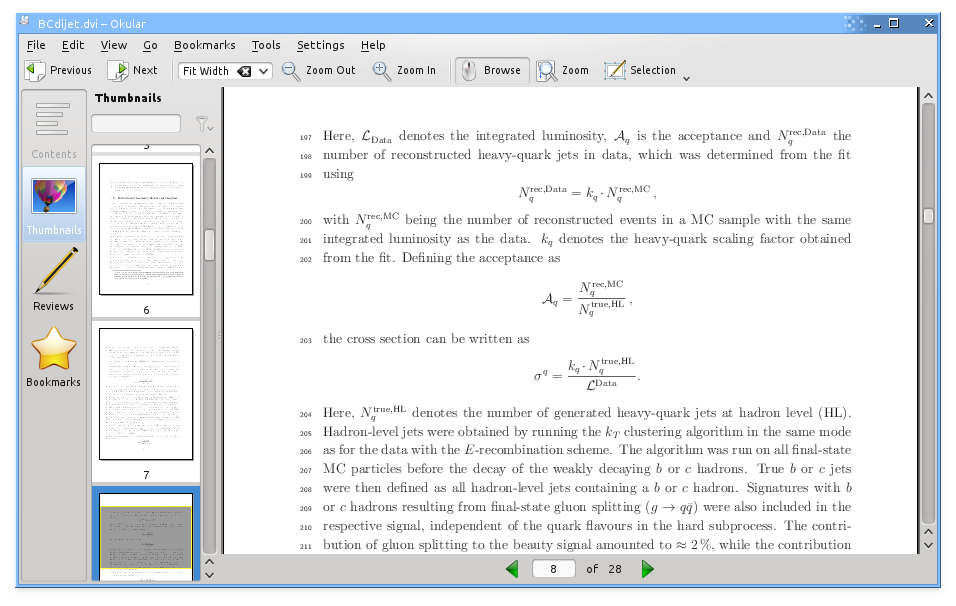
\includegraphics[width=7cm]{BCDijet-linenomath}\\
  (a) & (b)
  \end{tabular}
  \caption{Example of (a) a problem with line numbers and (b) its solution.}
  \label{fig:lineno}
\end{figure}

Such problems are associated with text that is close to math mode
environments. Some of the problems can be solved by using a new
version of the lineno package.
However, this only works for \enquote{standard} \LaTeX{}
math environments: \Env{displaymath}, \Env{equation} and \Env{eqnarray}, while it does
not work for recommended \Package{amsmath} environments such as \Env{equation*},
\Env{align(*)} and \Env{alignat(*)}.

The solution is to enclose the equation in \Env{linenomath} environment, e.g.
\begin{verbatim}
The total visible cross section for inclusive heavy-quark jet
production, $\sigma^{q}$, with $q\in\{b,c\}$ is given by
\begin{linenomath}
\begin{equation*}
  \sigma^{q} = \frac{N_{q}^{\text{rec,Data}}}{\mathcal{A}_{q}\cdot\mathcal{L}_{\text{Data}}}.
\end{equation*}
end{linenomath}
Here, $\mathcal{L}_{\text{Data}}$ denotes the integrated luminosity,
$\mathcal{A}_{q}$ is the acceptance and $N_{q}^{\text{rec,Data}}$ the
number of reconstructed heavy-quark jets in data, which was determined
\end{verbatim}

Then the line numbering will be correct, see Fig.~\ref{fig:lineno}b.

%%% Local Variables:
%%% mode: latex
%%% TeX-master: "../thesis_guide"
%%% End:
